\section{Benchmark and identification protocol}\label{sec:bench}

\subsection{Levels of the benchmark}\label{sec:levels}

The benchmark separates hiddenness from rarity and covers the types of systems for which heuristics have been proposed (\cref{tab:benchmark}; equations, parameters, and portraits in Section~\ref{app:systems}).
\textbf{Level A, three-dimensional flows:} the Chua circuit with two parameter sets~\cite{Leonov2011PLA,GuanXie2025,Kuznetsov2023Chua}; systems without equilibria, NE4, Wang--Chen \#1, and Wei~\cite{Wei2011,JafariSprottGolpayegani2013}, and the 2026 system of Jafari et al.\ without fixed points or perpetual points~\cite{Jafari2026NoPP}; systems with a single stable equilibrium, Wang--Chen \#2, SE3, and SE11~\cite{WangChen2012,Molaie2013}; LE1 with a line of equilibria~\cite{JafariSprott2013}; and the Rabinovich system~\cite{Kuznetsov2018Rabinovich}. The negative controls are the transient chaos of the Lorenz system at $(a,r,b)=(4,29,2)$~\cite{YorkeYorke1979} and the transient set of the Rabinovich system at $r=6.8$~\cite{SprottMunmuangsaen2018Comment}.
\textbf{Level B, maps:} the map of Huynh et al.\ without fixed points~\cite{Huynh2019}, eight cases of the family of Jiang et al.~\cite{Jiang2016Maps}, three parameter sets in the form of~\cite{Ouannas2018}, and the H\'enon map as a control.
\textbf{Level C, four-dimensional systems:} the simplified Lorenz system of Li and Sprott without equilibria~\cite{LiSprott2014} and the system of Jahanshahi et al.~\cite{Jahanshahi2019}, used for the census and the protocol.
\textbf{Level D:} synthetic families with analytically known basin measure (\cref{sec:synth}).
The region $B$ for three-dimensional flows is the cube $[-10,10]^3$, the natural region of the original publications; for the Chua circuit, it is $[-10,10]^2\times[-15,15]$, as in~\cite{Zelinka2016}. Basin fractions are estimated from $5\times10^4$ uniform points for most level-A systems and $2\times10^4$ otherwise; for the Chua circuit, they were checked independently with Attractors.jl~\cite{Datseris2018JOSS,DatserisWagemakers2022}.

\Cref{tab:benchmark} confirms that hiddenness and rarity differ. In the Rabinovich system and in Wang--Chen \#2, the hidden attractor occupies 76\% and 67\% of the region, respectively; only the targets of Chua~II, SE11, LE1, the Jafari cycle and chaos, and the Huynh map are rare ($p<10^{-2}$). The Jiang maps, characterized in~\cite{Jiang2016Maps} as having tiny basins, give $p\approx0.03$--$0.10$ in boxes around the attractors. The classical heuristics behave as described in~\cite{GuanXie2025}; on the rare targets SE11 and LE1, the best of them, sampling on nullclines, raises the hit frequency by factors of only 1.1 and 2.6 (Section~\ref{app:classic}). The literature baseline for the search experiments is differential evolution (DE) over initial conditions with the cost function of~\cite{Zelinka2016}; unlike our strategies, DE is given the size of the target.

The attractor of LE1 is hidden only in a weak sense. Trajectories started near the stable part of its line of equilibria ($z<0$) never reach it, but trajectories started at distance $10^{-8}$ from the unstable equilibria $(0,0,z_0)$ with $0.35\le z_0\le2.2$ do: 170 of 3360 starts on a grid of $z_0\in[-3,4]$ (Section~\ref{app:verification}). Jafari and Sprott, who introduced the system, also describe the attractor as hidden in a computational sense~\cite{JafariSprott2013}. We keep LE1 in the benchmark as a rare target: the cost of finding it from uniformly distributed initial conditions does not depend on how it is classified.

\begin{table}[tbhp]
\caption{Benchmark: search targets (hidden attractors), basin measures $p$ in the region $B$, and the cost of uniform sampling $N^0_{0.9}$ (0.9 quantile of the first-hit index over $R=50$ runs, $R=20$ for the Jafari chaos; for nonrare targets, $\lceil\ln0.1/\ln(1-p)\rceil$). A slash separates two symmetric attractors, and a semicolon separates different targets; ``both'' is the cost of hitting either. Here $\lambda$ is the largest Lyapunov exponent.}
\label{tab:benchmark}
\centering\scriptsize
\setlength{\tabcolsep}{3pt}
\begin{tabular}{l>{\raggedright\arraybackslash}p{2.6cm}>{\raggedright\arraybackslash}p{2.6cm}>{\raggedright\arraybackslash}p{1.9cm}>{\raggedright\arraybackslash}p{1.9cm}>{\raggedright\arraybackslash}p{1.3cm}}
\toprule
Level & System & Equilibria & Target & $p$ & $N^0_{0.9}$ \\
\midrule
A & Chua I & F$_0$ stable, F$_\pm$ saddle-foci & two chaotic & 0.017 / 0.018 & 136 / 124 \\
 & Chua II & F$_0$ saddle-focus, F$_\pm$ stable & cycle; two chaotic & 0.992; 0.0014 / 0.0013 & 1; 772 (both) \\
 & NE4 & none & chaos ($\lambda\approx0.03$) & 0.33 & 6 \\
 & Wang--Chen \#1 & none & chaos & 0.103 & 22 \\
 & Wei (NE2) & none & chaos & 0.096 & 23 \\
 & Jafari 2026, $a_3=-1$ & none; no perpetual points & cycle & 0.009 & 229 \\
 & Jafari 2026, $a_3=-3.548$ & none & fragile chaos & $(2$--$5)\times10^{-4}$ & 5331 \\
 & Wang--Chen \#2 & one, stable & chaos & 0.666 & 3 \\
 & SE3 & one, stable & chaos & 0.153 & 14 \\
 & SE11 & one, stable & chaos & 0.0079 & 302 \\
 & LE1 & line $x=y=0$, stable for $z<0$ & chaos (weakly hidden) & 0.0016 & 1422 \\
 & Rabinovich, $r=100$ & saddle, two stable foci & chaos & 0.763 & 2 \\
\midrule
B & Huynh 2019 & none & chaos & 0.0091 & 211 \\
 & Jiang 2016, NF I e--i & none & chaos & 0.028--0.039 & 59--82 \\
 & Jiang 2016, SF I a--d & one, stable & chaos & 0.065--0.10 & 22--35 \\
\midrule
C & Li--Sprott 4D, $a=6$ & none & torus; two strange & 0.090; 0.446 / 0.464 & 25; 4 \\
\midrule
D & D1, D2 (base SE3) & as for the base & chaos of the base & $10^{-2}$--$10^{-7}$ & 258--$2.1\times10^{7}$ \\
\bottomrule
\end{tabular}
\end{table}

\subsection{Synthetic families with known basin measure}\label{sec:synth}

To measure the scaling of the cost for $p$ down to $10^{-7}$ and dimensions up to 14, the system SE3 ($p_W=0.153$ in $[-10,10]^3$, where $W_{\rm HA}$ denotes its basin) is embedded in $\mathbb{R}^{3+m}$ with $B=[-10,10]^3\times[-1,1]^m$, in two constructions with opposite properties.
\textbf{D1, embedding with a gate,} has no transient signal:
\begin{equation}
\begin{gathered}
\dot x=F(x)-g(w)\,(x-e),\qquad \dot w=-\kappa w,\\
g(w)=\frac{H}{1+\exp\bigl(-400(|w|-\rho)/\rho\bigr)},
\end{gathered}
\label{eq:d1}
\end{equation}
where $e$ is the stable equilibrium of the base system, $H=50$, and $\kappa=0.5$. While $|w|>\rho$, the gate pulls $x$ toward $e$, so the basin is approximately $W_{\rm HA}\times\{|w_0|\le\rho\}$ and
\begin{equation}
p(\rho,m)=p_W\,\frac{V_m(\rho)}{2^m},\qquad V_m(\rho)=\frac{\pi^{m/2}\rho^m}{\Gamma(m/2+1)};
\label{eq:pD}
\end{equation}
the measured fractions agree with \eqref{eq:pD} to within 2\%--17\%. Outside a thin rim of the ball, the transient hardly depends on $|w_0|$.
\textbf{D2, edge state,} has a signal on all scales:
\begin{equation}
\dot x=F(x),\qquad \dot w=\kappa\, w\,\bigl(|w|^2/\rho^2-1\bigr),\qquad \kappa=1.
\label{eq:d2}
\end{equation}
The sphere $|w|=\rho$ is repelling; for $|w_0|<\rho$, $w$ decays, and for $|w_0|>\rho$, $|w|$ blows up in finite time. The target basin is exactly $W_{\rm HA}\times\{|w_0|<\rho\}$, \eqref{eq:pD} is exact given $p_W$, and the escape time for $|w_0|=\rho(1+\Delta)$ is $\ln\bigl((1+\Delta)^2/((1+\Delta)^2-1)\bigr)/(2\kappa)\approx\ln(1/2\Delta)/(2\kappa)$, which diverges at the basin boundary (\cref{fig:d2mech}), as it does for edge states of real systems~\cite{Vollmer2009Edge,LucariniBodai2017}.

\begin{figure}[tbhp]
\centering
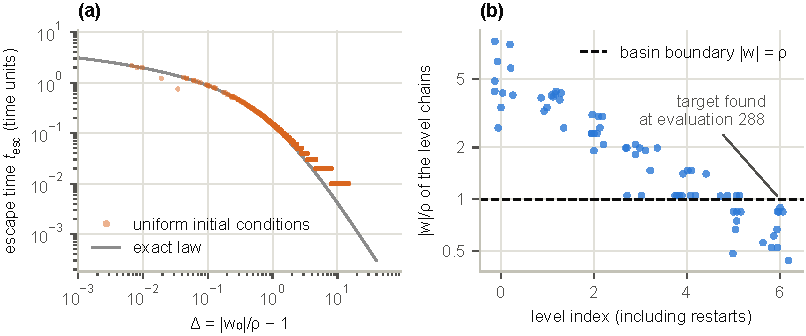
\includegraphics[width=\textwidth]{fig37_d2_mechanism.pdf}
\caption{Mechanism of the splitting gain in family D2 ($n=6$, $p=10^{-4}$). (a) Escape time versus the relative distance to the basin boundary $\Delta=|w_0|/\rho-1$ for $3\times10^4$ uniform initial conditions; the line is the exact law. The staircase on the right reflects the finite integration step. (b) $|w|/\rho$ for the seeds of the chains over the levels of one run; the chains contract into the ball $|w|<\rho$, and the target is found after 288 integrations, whereas uniform sampling needs $N^0_{0.9}=1.7\times10^4$.}
\label{fig:d2mech}
\end{figure}

\subsection{Identification and verification protocol}\label{sec:protocol}

Each trajectory is integrated with a fixed step by the fourth-order Runge--Kutta method (RK4; maps are iterated) over the transient segment and the observation window; escape is detected when $|x|>R_{\rm esc}$. Over the observation window, we compute the largest Lyapunov exponent $\lambda$ by the two-trajectory method~\cite{Benettin1980}, the mean speed, the maximum norm, the frequency of local maxima, the amplitude contraction ratio, and coordinate-wise means, standard deviations, minima, and maxima; the same statistics computed over an early window enter $\xi$. The kernels are implemented in Numba~\cite{Lam2015Numba}. The template of a regime consists of the mean $\bar f$ and the spread $\hat\sigma$ of the fingerprint over 64 copies started from random points of a segment on the attractor with relative noise $10^{-3}$; a trajectory with fingerprint $f$ is assigned to the template with the smallest
\begin{equation}
z=\max_i\frac{|f_i-\bar f_i|}{\hat\sigma_i+0.02\,(1+|\bar f_i|)},
\label{eq:z}
\end{equation}
provided that $z<6$ and the classes are compatible (a chaotic template requires $\lambda>0.005$, a regular one $\lambda<0.02$). Converged trajectories are compared with equilibria by their final points. Unmatched trajectories are clustered, and a new template is calibrated for each cluster; this is how unknown regimes are discovered.

Each candidate undergoes four checks: the lifetime (at least 20 windows, and up to $10^4$--$10^5$ time units for claims of a chaotic attractor), convergence in the step size (the same template and stable basin fractions under $\Delta t\to\Delta t/2$), an independent integrator (DOP853~\cite{Hairer1993} with $\mathrm{rtol}=10^{-11}$ and Attractors.jl), and the sign of $\lambda$ over consecutive windows. For claims of hiddenness, $h_\varepsilon$ is estimated by sampling in the $\varepsilon$-neighborhoods of all equilibria and along their unstable manifolds, $\varepsilon\in\{10^{-3},10^{-2},10^{-1}\}L$. The protocol was refined on three cases that would change the conclusions if missed (Section~\ref{app:verification}): numerical transient chaos of the Chua circuit at $\Delta t=0.01$, which causes the fractions of the hidden attractors to be underestimated almost twofold; a published table of basin fractions whose hidden-attractor fractions coincide with ours only at that coarse step; and intermittency and long-lived transient sets mistaken for attractors. The step-convergence and lifetime checks are therefore mandatory.
